\section{Randomized Algorithm}

This section describes a randomized algorithm designed to find a vertex cover of size \( k \) in an undirected graph \( G(V, E) \). The algorithm employs a probabilistic approach to select vertices that could potentially form a vertex cover.


\subsection{Algorithm Description}

The algorithm begins by initializing an empty set \( \text{{vertex\_cover}} \) and a copy of the original graph \( \text{{remaining\_graph}} \). It also maintains a set \( \text{{added\_vertices}} \) to track vertices already added to the vertex cover. The algorithm runs until the size of \( \text{{vertex\_cover}} \) reaches \( k \) or there are no more edges in \( \text{{remaining\_graph}} \).

In each iteration, the algorithm selects a random edge from \( \text{{remaining\_graph}} \) and then randomly chooses one of its vertices. If this vertex is not already in \( \text{{added\_vertices}} \), it is added to both \( \text{{vertex\_cover}} \) and \( \text{{added\_vertices}} \). Subsequently, all edges connected to this vertex are removed from \( \text{{remaining\_graph}} \).

The algorithm returns the vertex cover if it successfully reduces \( \text{{remaining\_graph}} \) to have no edges and \( \text{{vertex\_cover}} \) is of size \( k \). Otherwise, it returns None. It also tracks the number of operations, the execution time, and the number of solutions tested.

\subsection{Pseudocode}

\begin{algorithm}
\caption{Randomized FPT}
\begin{algorithmic}[1]

\Procedure{randomized\_fpt}{$graph, k$}
\State $vertex\_cover \gets \text{set}()$
\State $remaining\_graph \gets graph.copy()$
\State $added\_vertices \gets \text{set}()$
\While{$\text{len}(vertex\_cover) < k$}
\If{$\text{len}(remaining\_graph.edges()) = 0$}
\State \textbf{break}
\EndIf
\State $graph\_edges \gets \text{list}(remaining\_graph.edges())$
\State $edge \gets \text{random.choice}(graph\_edges)$
\State $vertex \gets \text{random.choice}(edge)$
\If{$vertex \in added\_vertices$}
\State \textbf{continue}
\EndIf
\State $vertex\_cover.add(vertex)$
\State $added\_vertices.add(vertex)$
\State $edges\_to\_remove \gets [e \text{ for } e \text{ in } remaining\_graph.edges(vertex)]$
\State $remaining\_graph.remove\_edges\_from(
edges\_to\_remove)$
\EndWhile
\If{$\text{len}(remaining\_graph.edges()) = 0$ \textbf{and} $\text{len}(vertex\_cover) = k$}
\State \Return $vertex\_cover$
\Else
\State \Return $\text{None}$
\EndIf
\EndProcedure
\end{algorithmic}
\end{algorithm}


\subsection{Formal Analysis}
The time complexity of the randomized vertex cover algorithm can be approximated as \(O(k \cdot m)\), where \(k\) is the size of the desired vertex cover, and \(m\) is the number of edges. In each iteration, the algorithm randomly selects an edge and then a vertex from this edge, removing all edges incident to this vertex. This process is repeated up to \(k\) times or until no more edges remain.

In terms of complexity analysis:
\begin{itemize}
  \item \textbf{Best Case:} The best case occurs when the algorithm efficiently finds a vertex cover that covers all edges early in the process. This scenario's complexity can be better than \(O(k \cdot m)\), depending on the graph's structure and the randomness of the selections.
  
  \item \textbf{Average Case:} The average case complexity remains at \(O(k \cdot m)\). On average, the algorithm may require several iterations to find an effective vertex cover, with each iteration involving random edge and vertex selections and edge removals.
  
  \item \textbf{Worst Case:} The worst case occurs when the algorithm iterates \(k\) times, each time dealing with a significant number of edges. Thus, the time complexity is \(O(k \cdot m)\).
\end{itemize}

\subsection{Experimental Analysis}
To empirically assess the algorithm's performance, it was tested on randomly generated graphs with varying numbers of vertices and edges. The parameters were:

\begin{itemize}
    \item \(n\) (number of vertices) Range: From 4 to 256, to cover a broad spectrum of graph sizes.
    \item \(m\) (number of edges) Proportions: Fixed percentages of the maximum possible number of edges, specifically \{0.125, 0.25, 0.5, 0.75\} of the maximum.
    \item \(k\) (vertex cover size) Proportions: Relative to the number of vertices, with proportions \{0.125, 0.25, 0.5, 0.75\}.
\end{itemize}

Two metrics were evaluated:\begin{enumerate}
    \item Number of Basic Operations: Operations for each random selection of edges and vertices, and for edge removals.
    \item Number of Solutions Tested: Total number of vertex cover sets attempted until the algorithm terminates.
\end{enumerate}

For the analysis, we focused on the first iteration, showing different comparisons across different \(k\) percentages.

\subsubsection{Analysis of Operations}

The number of operations required by the algorithm shows distinct growth patterns that vary with the edge density and vertex cover size. Figure \ref{fig:ops_12_5_first} and \ref{fig:ops_75_first} depict the operations for the first iteration.

\begin{figure}[h]
\centering
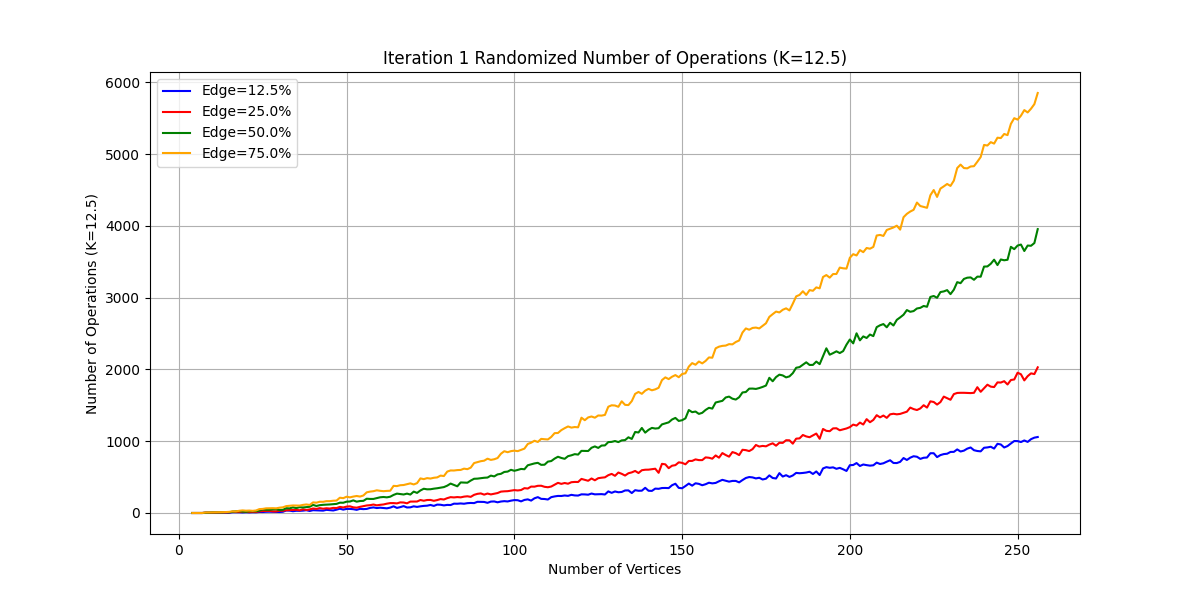
\includegraphics[width=0.5\textwidth]{FPT/Number of Operations (K=12.5).png}
\caption{FPT \(|\) Number of operations for \( K=12.5 \).}
\label{fig:ops_12_5_first}
\end{figure}

\begin{figure}[h]
\centering
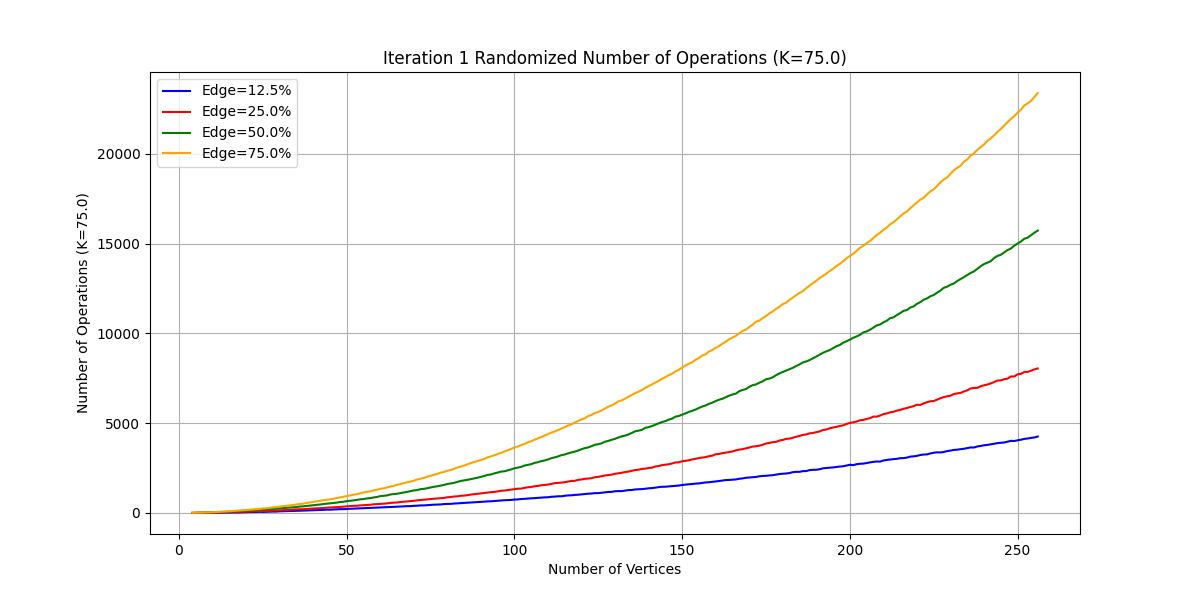
\includegraphics[width=0.5\textwidth]{FPT/Number of Operations (K=75.0).png}
\caption{FPT \(|\) Number of operations for \( K=75.0 \).}
\label{fig:ops_75_first}
\end{figure}

\subsubsection{Analysis of Solutions Tested}

Similarly, the number of solutions tested is depicted in Figures \ref{fig:sol_12_5_first} and \ref{fig:sol_75_first} for the first iteration.

\begin{figure}[h]
\centering
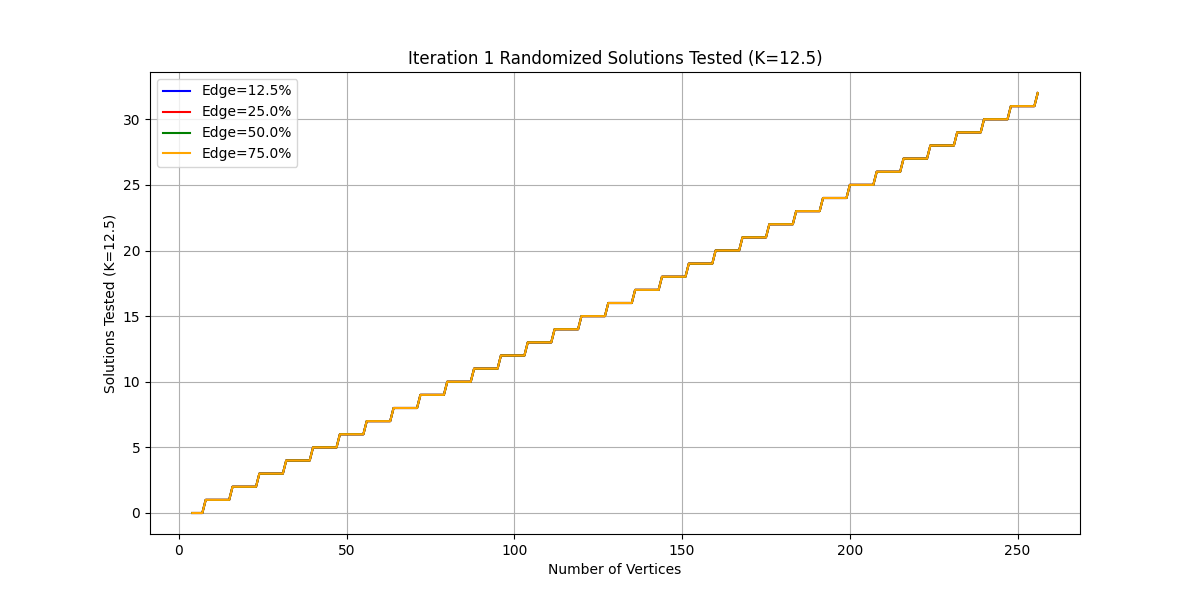
\includegraphics[width=0.5\textwidth]{FPT/Solutions Tested (K=12.5).png}
\caption{FPT \(|\) Number of solutions tested for \( K=12.5 \).}
\label{fig:sol_12_5_first}
\end{figure}

\begin{figure}[h]
\centering
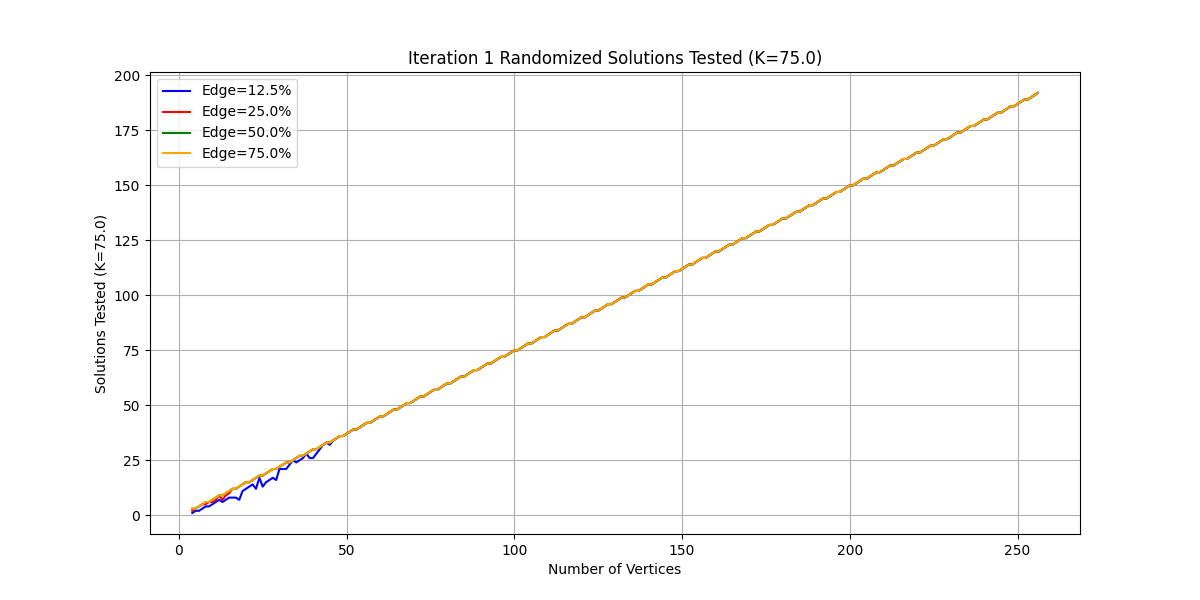
\includegraphics[width=0.5\textwidth]{FPT/Solutions Tested (K=75.0).png}
\caption{FPT \(|\) Number of solutions tested for \( K=75.0 \).}
\label{fig:sol_75_first}
\end{figure}

\subsubsection{Comparative Conclusions}

Upon comparing the figures, it becomes evident that the algorithm's behavior maintains consistency in terms of the number of solutions tested, which appears to grow linearly as seen in Figures \ref{fig:sol_12_5_first} to \ref{fig:sol_75_first}. However, a different pattern emerges when analyzing the number of operations. While the operations for \( K=12.5 \) exhibit a growth that could be interpreted as polynomial (Figure \ref{fig:ops_12_5_first}), the operations for \( K=75.0 \) suggest a steeper, possibly exponential increase (Figure \ref{fig:ops_75_first}). This steepening trend for larger vertex covers implies that the algorithmic complexity is significantly affected by the vertex cover size sought.

The edge density also plays a crucial role. Higher edge densities lead to more complex graphs, which in turn require more operations, highlighting the non-linear impact of graph density on the computational workload.

Overall, the data suggests that while the number of solutions tested remains relatively stable and linear, the operations required by the algorithm for larger vertex covers and denser graphs could be subject to exponential increases in complexity. This underlines the importance of considering both the vertex cover size and edge density when assessing the performance and scalability of such randomized algorithms, however this algorithm very rarely finds a solution. This problem will be talked about more in the following sections.
